\documentclass[12pt,hyperref,a4paper,UTF8]{ctexart}
\usepackage{HDUReport}
\usepackage{listings}
\usepackage{xcolor}
\usepackage{graphicx}
\usepackage{setspace}
\usepackage{float}
\setstretch{1.5} % 设置全局行距为1.5倍

\usepackage{enumitem} % 载入enumitem包以便自定义列表环境
\setlist[itemize]{itemsep=0pt, parsep=0pt} % 设置itemize环境的项目间距和段落间距

\setmainfont{Times New Roman} % 英文正文为Times New Roman


\usepackage{tikz}
\usetikzlibrary{shapes.geometric, arrows}
\usetikzlibrary{positioning, arrows.meta}
\usetikzlibrary{calc}
%封面页设置
{   
    %标题
    \title{ 
        \vspace{1cm}
        \heiti \Huge \textbf{《单片机原理及应用》作业报告} \par
        \vspace{1cm} 
        \heiti \Large {\underline{实验报告4第二部分:数码管显示步进}   } 
        \vspace{3cm}
    
    }

    \author{
        \vspace{0.5cm}
        \kaishu\Large 学院\ \dlmu[9cm]{卓越学院} \\ %学院
        \vspace{0.5cm}
        \kaishu\Large 学号\ \dlmu[9cm]{23040447} \\ %班级
        \vspace{0.5cm}
        \kaishu\Large 姓名\ \dlmu[9cm]{陈文轩} \qquad  \\ %学号
        \vspace{0.5cm}
        \kaishu\Large 专业\ \dlmu[9cm]{智能硬件与系统(电子信息工程)} \qquad \\ %姓名 
    }
        
    \date{\today} % 默认为今天的日期,可以注释掉不显示日期
}
%%------------------------document环境开始------------------------%%
\begin{document}

%%-----------------------封面--------------------%%
\cover
\thispagestyle{empty} % 首页不显示页码
%%------------------摘要-------------%%
%\newpage
%\begin{abstract}




%\end{abstract}

%\thispagestyle{empty} % 首页不显示页码

%%--------------------------目录页------------------------%%
% \newpage
% \tableofcontents
% \thispagestyle{empty} % 目录不显示页码

%%------------------------正文页从这里开始-------------------%
\newpage
\setcounter{page}{1} % 让页码从正文开始编号

%%可选择这里也放一个标题
%\begin{center}
%    \title{ \Huge \textbf{{标题}}}
%\end{center}


\textbf{在LED显示器上显示4位10进制数,设置4个按键,按键每按一次,对应的位数上的数值加1。}


\section{实验代码}

\begin{lstlisting}[language=C, caption={实验程序}]

#include <reg51.h> // 单片机头文件

unsigned char code Tab[] = {0xC0, 0xF9, 0xA4, 0xB0, 0x99, 0x92, 0x82, 0xF8, 0x80, 0x90}; // 共阳数码管码段表
unsigned char Dat[] = {0, 0, 0, 0}; // 存放4位数字数组

int i; // 定义变量,作为循环
unsigned char tmp; // 定义片选变量

unsigned char KeyState = 0x0F; // 按键状态变量,初始值为高电平(未按下)

#define KEY1 (P1 & 0x01) // 按键1连接到 P1.0
#define KEY2 (P1 & 0x02) // 按键2连接到 P1.1
#define KEY3 (P1 & 0x04) // 按键3连接到 P1.2
#define KEY4 (P1 & 0x08) // 按键4连接到 P1.3

void Delay() // 延时子程序,作为数码管显示延迟
{
    unsigned char i;
    for (i = 0; i < 250; i++);
}

void ScanKeys() // 按键扫描函数
{
    // 检测按键1(P1.0)
    if ((KeyState & 0x01) && !KEY1) // 上一次状态为高电平,当前为低电平
    {
        Delay(); // 消抖
        if (!KEY1) // 再次确认按键按下
        {
            Dat[0] = (Dat[0] + 1) % 10; // 第一位数字加1
        }
    }
    KeyState = (KeyState & ~0x01) | (KEY1 ? 0x01 : 0x00); // 更新按键1状态

    // 检测按键2(P1.1)
    if ((KeyState & 0x02) && !KEY2) // 上一次状态为高电平,当前为低电平
    {
        Delay(); // 消抖
        if (!KEY2) // 再次确认按键按下
        {
            Dat[1] = (Dat[1] + 1) % 10; // 第二位数字加1
        }
    }
    KeyState = (KeyState & ~0x02) | (KEY2 ? 0x02 : 0x00); // 更新按键2状态

    // 检测按键3(P1.2)
    if ((KeyState & 0x04) && !KEY3) // 上一次状态为高电平,当前为低电平
    {
        Delay(); // 消抖
        if (!KEY3) // 再次确认按键按下
        {
            Dat[2] = (Dat[2] + 1) % 10; // 第三位数字加1
        }
    }
    KeyState = (KeyState & ~0x04) | (KEY3 ? 0x04 : 0x00); // 更新按键3状态

    // 检测按键4(P1.3)
    if ((KeyState & 0x08) && !KEY4) // 上一次状态为高电平,当前为低电平
    {
        Delay(); // 消抖
        if (!KEY4) // 再次确认按键按下
        {
            Dat[3] = (Dat[3] + 1) % 10; // 第四位数字加1
        }
    }
    KeyState = (KeyState & ~0x08) | (KEY4 ? 0x08 : 0x00); // 更新按键4状态
}

void main()
{
    while (1) // 无限循环
    {
        ScanKeys(); // 调用按键扫描函数

        tmp = 0x01; // 片选初值
        for (i = 0; i < 4; i++) // 循环4次
        {
            P2 = tmp; // 片选初值
            P0 = Tab[Dat[i]]; // 输出某一位数字的码段值
            tmp = tmp << 1; // 片选值左移一位
            Delay(); // 调用延时
        }
    }
}

\end{lstlisting}

\section{实验效果}

\begin{figure}[H] % [H] 表示强制当前位置插入
    \centering
    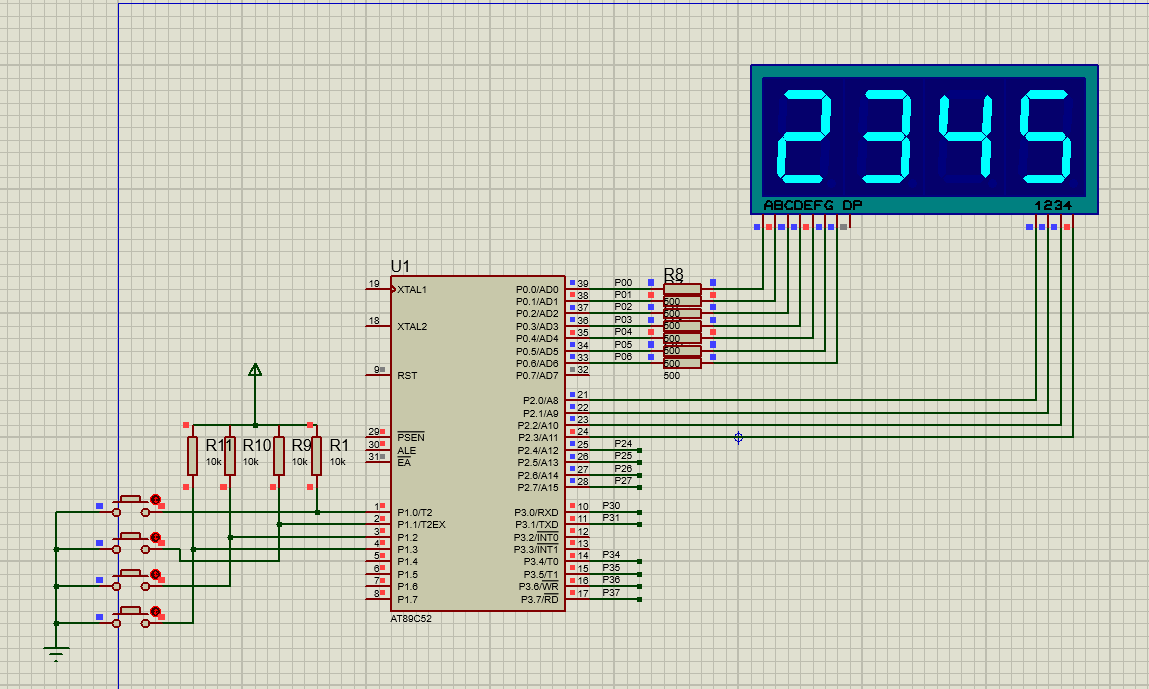
\includegraphics[width=0.9\textwidth]{figures/201.png} % 调整宽度为文本宽度的 80%
    \caption{2345显示效果 } %图片标题
    \label{fig:example} % 图片标签,用于引用
\end{figure}

\begin{figure}[H] % [H] 表示强制当前位置插入
    \centering
    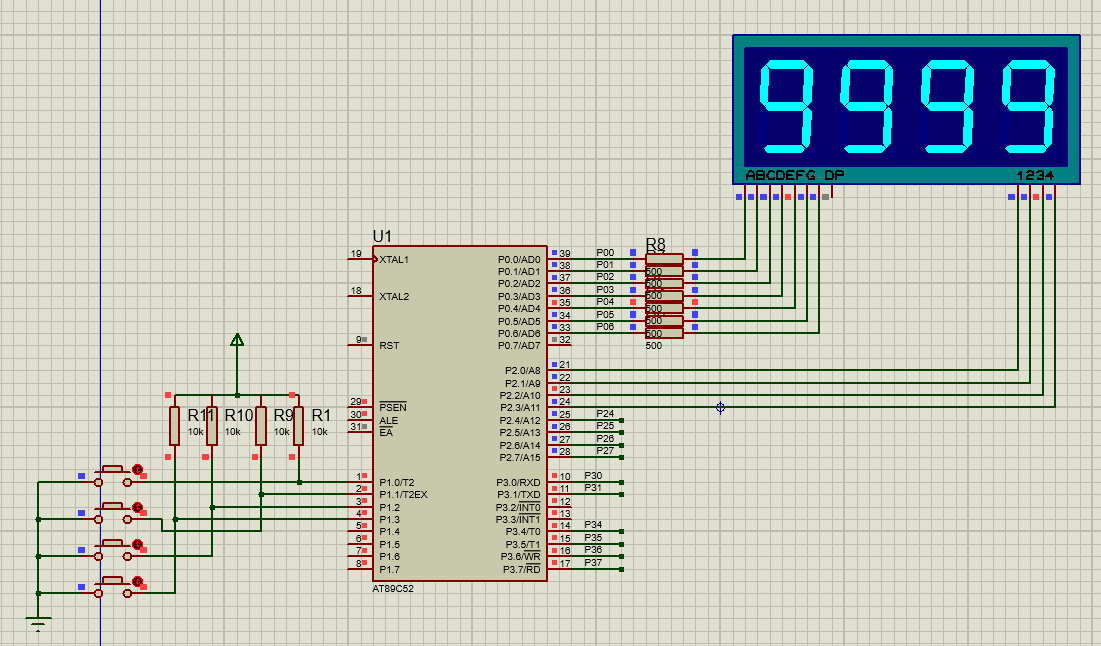
\includegraphics[width=0.9\textwidth]{figures/202.png} % 调整宽度为文本宽度的 80%
    \caption{9999显示效果 } %图片标题
    \label{fig:example} % 图片标签,用于引用
\end{figure}

\begin{figure}[H] % [H] 表示强制当前位置插入
    \centering
    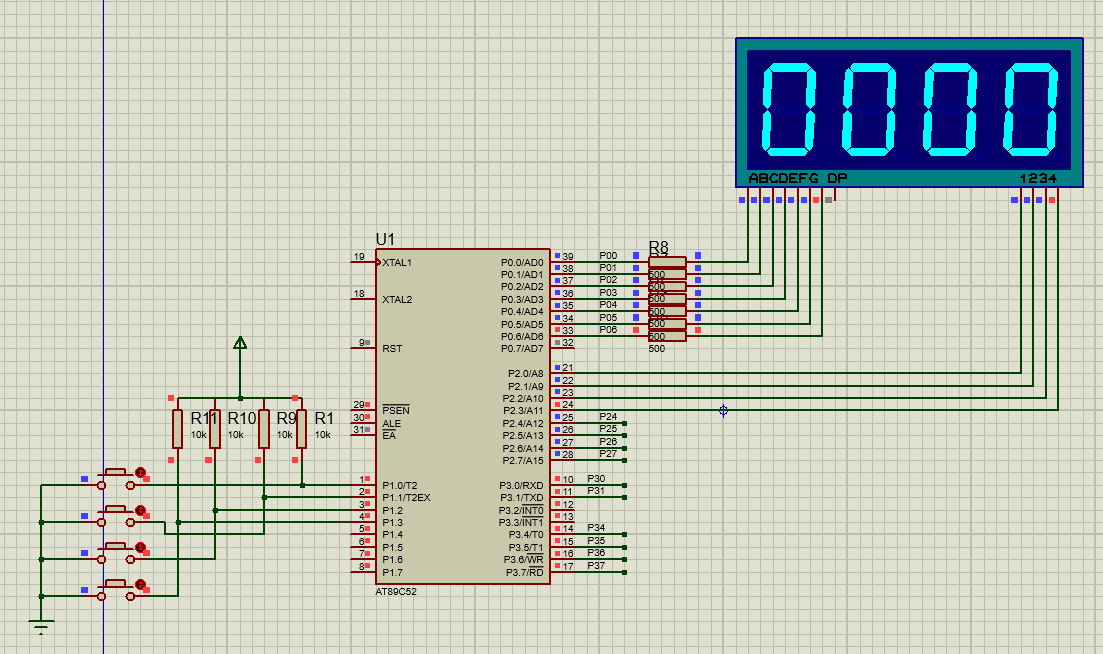
\includegraphics[width=0.9\textwidth]{figures/203.png} % 调整宽度为文本宽度的 80%
    \caption{0000显示效果 } %图片标题
    \label{fig:example} % 图片标签,用于引用
\end{figure}


\section{流程图}


\begin{figure}[H] % [H] 表示强制当前位置插入
        \centering
        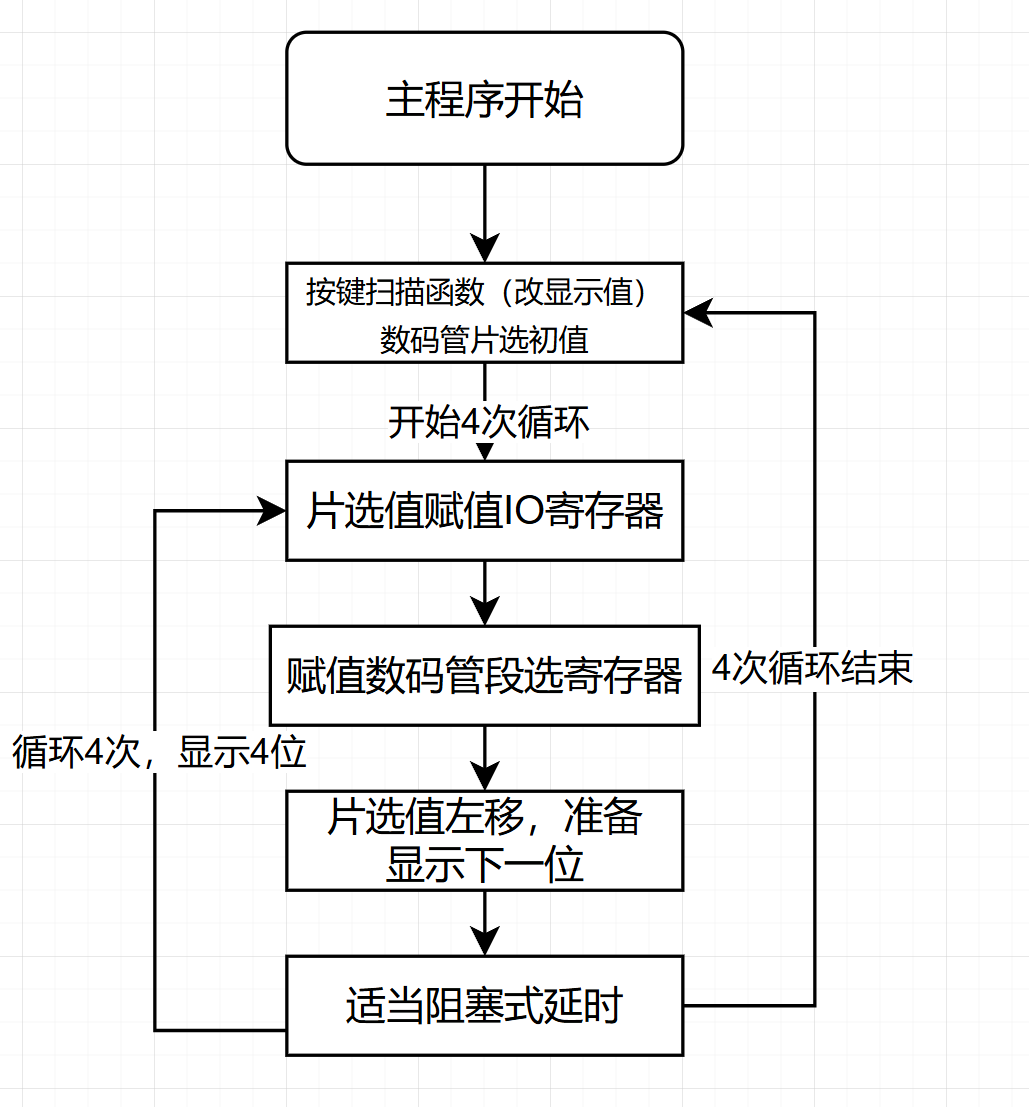
\includegraphics[width=0.9\textwidth]{figures/301.png} % 调整宽度为文本宽度的 80%
        \caption{系统控制流程图} %图片标题
        \label{fig:example} % 图片标签,用于引用
\end{figure}



\section{实验体会}


本实验通过动态扫描方式实现了按键扫描(状态机边沿检测)、数码管显示(基于阻塞形式的延时)等功能,进一步加深了数码管的应用原理的相关理解,同时体验了按键扫描的常规过程,对日后的单片机开发积累了经验。



\end{document}